

\tikzset{every picture/.style={line width=0.75pt}} %set default line width to 0.75pt        

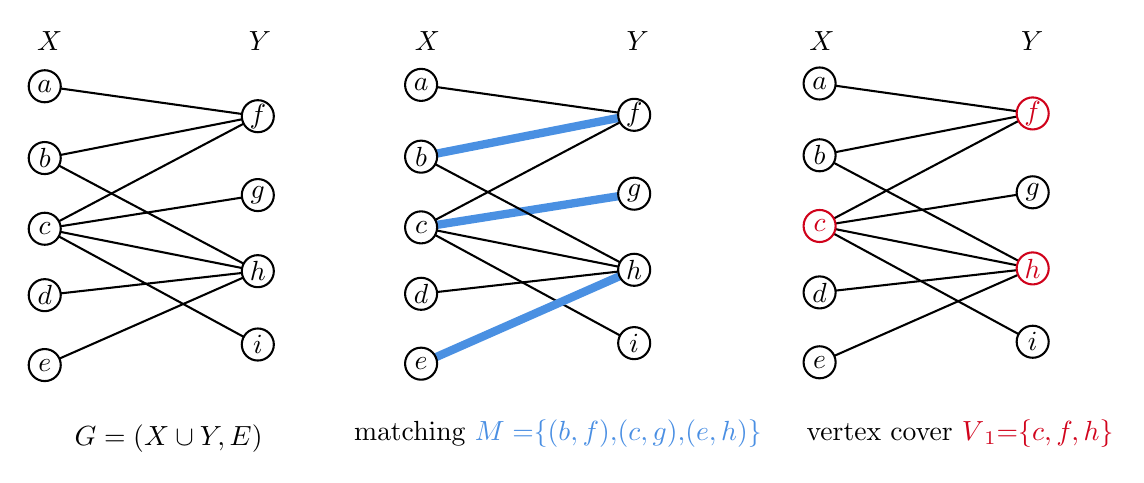
\begin{tikzpicture}[x=0.5pt,y=0.5pt,yscale=-1,xscale=1]
%uncomment if require: \path (0,316); %set diagram left start at 0, and has height of 316

%Straight Lines [id:da6233481480623783] 
\draw    (173.67,69.73) -- (19.68,99.97) ;
%Straight Lines [id:da3790939323014558] 
\draw    (19.68,48.09) -- (173.67,69.73) ;
%Straight Lines [id:da555393377892622] 
\draw    (173.67,69.73) -- (19.68,151.07) ;
%Straight Lines [id:da17109149534540602] 
\draw    (173.67,181.73) -- (19.68,151.07) ;
%Straight Lines [id:da8491552224613422] 
\draw    (173.67,234.73) -- (19.68,151.07) ;
%Straight Lines [id:da6111412207445381] 
\draw    (173.67,126.73) -- (19.68,151.07) ;
%Straight Lines [id:da40246334963984653] 
\draw    (173.67,181.73) -- (19.68,199.07) ;
%Straight Lines [id:da8951096474536266] 
\draw    (173.67,181.73) -- (19.68,249.58) ;
%Straight Lines [id:da442507224234595] 
\draw    (173.67,181.73) -- (19.68,99.97) ;
%Shape: Ellipse [id:dp9133580928774087] 
\draw  [fill={rgb, 255:red, 255; green, 255; blue, 255 }  ,fill opacity=1 ] (8.1,249.58) .. controls (8.1,243.18) and (13.29,238) .. (19.68,238) .. controls (26.08,238) and (31.26,243.18) .. (31.26,249.58) .. controls (31.26,255.97) and (26.08,261.16) .. (19.68,261.16) .. controls (13.29,261.16) and (8.1,255.97) .. (8.1,249.58) -- cycle ;
%Shape: Ellipse [id:dp4005957609675306] 
\draw  [fill={rgb, 255:red, 255; green, 255; blue, 255 }  ,fill opacity=1 ] (8.1,99.97) .. controls (8.1,93.57) and (13.29,88.39) .. (19.68,88.39) .. controls (26.08,88.39) and (31.26,93.57) .. (31.26,99.97) .. controls (31.26,106.36) and (26.08,111.55) .. (19.68,111.55) .. controls (13.29,111.55) and (8.1,106.36) .. (8.1,99.97) -- cycle ;
%Shape: Ellipse [id:dp49214617921702164] 
\draw  [fill={rgb, 255:red, 255; green, 255; blue, 255 }  ,fill opacity=1 ] (8.1,151.07) .. controls (8.1,144.67) and (13.29,139.49) .. (19.68,139.49) .. controls (26.08,139.49) and (31.26,144.67) .. (31.26,151.07) .. controls (31.26,157.46) and (26.08,162.65) .. (19.68,162.65) .. controls (13.29,162.65) and (8.1,157.46) .. (8.1,151.07) -- cycle ;
%Shape: Ellipse [id:dp8440754424343925] 
\draw  [fill={rgb, 255:red, 255; green, 255; blue, 255 }  ,fill opacity=1 ] (8.1,199.07) .. controls (8.1,192.68) and (13.29,187.49) .. (19.68,187.49) .. controls (26.08,187.49) and (31.26,192.68) .. (31.26,199.07) .. controls (31.26,205.47) and (26.08,210.65) .. (19.68,210.65) .. controls (13.29,210.65) and (8.1,205.47) .. (8.1,199.07) -- cycle ;
%Shape: Ellipse [id:dp20660183368429152] 
\draw  [fill={rgb, 255:red, 255; green, 255; blue, 255 }  ,fill opacity=1 ] (8.1,48.09) .. controls (8.1,41.7) and (13.29,36.51) .. (19.68,36.51) .. controls (26.08,36.51) and (31.26,41.7) .. (31.26,48.09) .. controls (31.26,54.49) and (26.08,59.67) .. (19.68,59.67) .. controls (13.29,59.67) and (8.1,54.49) .. (8.1,48.09) -- cycle ;
%Shape: Ellipse [id:dp4098192910838151] 
\draw  [fill={rgb, 255:red, 255; green, 255; blue, 255 }  ,fill opacity=1 ] (162.09,69.73) .. controls (162.09,63.33) and (167.27,58.15) .. (173.67,58.15) .. controls (180.06,58.15) and (185.25,63.33) .. (185.25,69.73) .. controls (185.25,76.13) and (180.06,81.31) .. (173.67,81.31) .. controls (167.27,81.31) and (162.09,76.13) .. (162.09,69.73) -- cycle ;
%Shape: Ellipse [id:dp04818959761719954] 
\draw  [fill={rgb, 255:red, 255; green, 255; blue, 255 }  ,fill opacity=1 ] (162.09,126.73) .. controls (162.09,120.33) and (167.27,115.15) .. (173.67,115.15) .. controls (180.06,115.15) and (185.25,120.33) .. (185.25,126.73) .. controls (185.25,133.13) and (180.06,138.31) .. (173.67,138.31) .. controls (167.27,138.31) and (162.09,133.13) .. (162.09,126.73) -- cycle ;
%Shape: Ellipse [id:dp776083183452069] 
\draw  [fill={rgb, 255:red, 255; green, 255; blue, 255 }  ,fill opacity=1 ] (162.09,181.73) .. controls (162.09,175.33) and (167.27,170.15) .. (173.67,170.15) .. controls (180.06,170.15) and (185.25,175.33) .. (185.25,181.73) .. controls (185.25,188.13) and (180.06,193.31) .. (173.67,193.31) .. controls (167.27,193.31) and (162.09,188.13) .. (162.09,181.73) -- cycle ;
%Shape: Ellipse [id:dp943943166831801] 
\draw  [fill={rgb, 255:red, 255; green, 255; blue, 255 }  ,fill opacity=1 ] (162.09,234.73) .. controls (162.09,228.33) and (167.27,223.15) .. (173.67,223.15) .. controls (180.06,223.15) and (185.25,228.33) .. (185.25,234.73) .. controls (185.25,241.13) and (180.06,246.31) .. (173.67,246.31) .. controls (167.27,246.31) and (162.09,241.13) .. (162.09,234.73) -- cycle ;
%Straight Lines [id:da5762269873281055] 
\draw [color={rgb, 255:red, 74; green, 144; blue, 226 }  ,draw opacity=1 ][line width=3]    (445.67,68.73) -- (291.68,98.97) ;
%Straight Lines [id:da6557704374413869] 
\draw    (291.68,47.09) -- (445.67,68.73) ;
%Straight Lines [id:da37940197486810245] 
\draw    (445.67,68.73) -- (291.68,150.07) ;
%Straight Lines [id:da2489426088203095] 
\draw    (445.67,180.73) -- (291.68,150.07) ;
%Straight Lines [id:da614864797412136] 
\draw    (445.67,233.73) -- (291.68,150.07) ;
%Straight Lines [id:da19212175099205075] 
\draw [color={rgb, 255:red, 74; green, 144; blue, 226 }  ,draw opacity=1 ][line width=3]    (445.67,125.73) -- (291.68,150.07) ;
%Straight Lines [id:da318853764666447] 
\draw    (445.67,180.73) -- (291.68,198.07) ;
%Straight Lines [id:da3703675549768074] 
\draw [color={rgb, 255:red, 74; green, 144; blue, 226 }  ,draw opacity=1 ][line width=3]    (445.67,180.73) -- (291.68,248.58) ;
%Straight Lines [id:da8823098712187499] 
\draw    (445.67,180.73) -- (291.68,98.97) ;
%Shape: Ellipse [id:dp3095150063265397] 
\draw  [fill={rgb, 255:red, 255; green, 255; blue, 255 }  ,fill opacity=1 ] (280.1,248.58) .. controls (280.1,242.18) and (285.29,237) .. (291.68,237) .. controls (298.08,237) and (303.26,242.18) .. (303.26,248.58) .. controls (303.26,254.97) and (298.08,260.16) .. (291.68,260.16) .. controls (285.29,260.16) and (280.1,254.97) .. (280.1,248.58) -- cycle ;
%Shape: Ellipse [id:dp20721463292670939] 
\draw  [fill={rgb, 255:red, 255; green, 255; blue, 255 }  ,fill opacity=1 ] (280.1,98.97) .. controls (280.1,92.57) and (285.29,87.39) .. (291.68,87.39) .. controls (298.08,87.39) and (303.26,92.57) .. (303.26,98.97) .. controls (303.26,105.36) and (298.08,110.55) .. (291.68,110.55) .. controls (285.29,110.55) and (280.1,105.36) .. (280.1,98.97) -- cycle ;
%Shape: Ellipse [id:dp5446258401720914] 
\draw  [fill={rgb, 255:red, 255; green, 255; blue, 255 }  ,fill opacity=1 ] (280.1,150.07) .. controls (280.1,143.67) and (285.29,138.49) .. (291.68,138.49) .. controls (298.08,138.49) and (303.26,143.67) .. (303.26,150.07) .. controls (303.26,156.46) and (298.08,161.65) .. (291.68,161.65) .. controls (285.29,161.65) and (280.1,156.46) .. (280.1,150.07) -- cycle ;
%Shape: Ellipse [id:dp012444989815690533] 
\draw  [fill={rgb, 255:red, 255; green, 255; blue, 255 }  ,fill opacity=1 ] (280.1,198.07) .. controls (280.1,191.68) and (285.29,186.49) .. (291.68,186.49) .. controls (298.08,186.49) and (303.26,191.68) .. (303.26,198.07) .. controls (303.26,204.47) and (298.08,209.65) .. (291.68,209.65) .. controls (285.29,209.65) and (280.1,204.47) .. (280.1,198.07) -- cycle ;
%Shape: Ellipse [id:dp5639306398005206] 
\draw  [fill={rgb, 255:red, 255; green, 255; blue, 255 }  ,fill opacity=1 ] (280.1,47.09) .. controls (280.1,40.7) and (285.29,35.51) .. (291.68,35.51) .. controls (298.08,35.51) and (303.26,40.7) .. (303.26,47.09) .. controls (303.26,53.49) and (298.08,58.67) .. (291.68,58.67) .. controls (285.29,58.67) and (280.1,53.49) .. (280.1,47.09) -- cycle ;
%Shape: Ellipse [id:dp3692499940189833] 
\draw  [fill={rgb, 255:red, 255; green, 255; blue, 255 }  ,fill opacity=1 ] (434.09,68.73) .. controls (434.09,62.33) and (439.27,57.15) .. (445.67,57.15) .. controls (452.06,57.15) and (457.25,62.33) .. (457.25,68.73) .. controls (457.25,75.13) and (452.06,80.31) .. (445.67,80.31) .. controls (439.27,80.31) and (434.09,75.13) .. (434.09,68.73) -- cycle ;
%Shape: Ellipse [id:dp17469367724521878] 
\draw  [fill={rgb, 255:red, 255; green, 255; blue, 255 }  ,fill opacity=1 ] (434.09,125.73) .. controls (434.09,119.33) and (439.27,114.15) .. (445.67,114.15) .. controls (452.06,114.15) and (457.25,119.33) .. (457.25,125.73) .. controls (457.25,132.13) and (452.06,137.31) .. (445.67,137.31) .. controls (439.27,137.31) and (434.09,132.13) .. (434.09,125.73) -- cycle ;
%Shape: Ellipse [id:dp35472333728828986] 
\draw  [fill={rgb, 255:red, 255; green, 255; blue, 255 }  ,fill opacity=1 ] (434.09,180.73) .. controls (434.09,174.33) and (439.27,169.15) .. (445.67,169.15) .. controls (452.06,169.15) and (457.25,174.33) .. (457.25,180.73) .. controls (457.25,187.13) and (452.06,192.31) .. (445.67,192.31) .. controls (439.27,192.31) and (434.09,187.13) .. (434.09,180.73) -- cycle ;
%Shape: Ellipse [id:dp4084404782784946] 
\draw  [fill={rgb, 255:red, 255; green, 255; blue, 255 }  ,fill opacity=1 ] (434.09,233.73) .. controls (434.09,227.33) and (439.27,222.15) .. (445.67,222.15) .. controls (452.06,222.15) and (457.25,227.33) .. (457.25,233.73) .. controls (457.25,240.13) and (452.06,245.31) .. (445.67,245.31) .. controls (439.27,245.31) and (434.09,240.13) .. (434.09,233.73) -- cycle ;
%Straight Lines [id:da2461791334712684] 
\draw    (733.67,67.73) -- (579.68,97.97) ;
%Straight Lines [id:da45747325160291075] 
\draw    (579.68,46.09) -- (733.67,67.73) ;
%Straight Lines [id:da9670994187206017] 
\draw    (733.67,67.73) -- (579.68,149.07) ;
%Straight Lines [id:da75134152117505] 
\draw    (733.67,179.73) -- (579.68,149.07) ;
%Straight Lines [id:da3699894396868808] 
\draw    (733.67,232.73) -- (579.68,149.07) ;
%Straight Lines [id:da13352692532928045] 
\draw    (733.67,124.73) -- (579.68,149.07) ;
%Straight Lines [id:da12851059505065643] 
\draw    (733.67,179.73) -- (579.68,197.07) ;
%Straight Lines [id:da9630672080240875] 
\draw    (733.67,179.73) -- (579.68,247.58) ;
%Straight Lines [id:da43029644611033324] 
\draw    (733.67,179.73) -- (579.68,97.97) ;
%Shape: Ellipse [id:dp8625040314784665] 
\draw  [fill={rgb, 255:red, 255; green, 255; blue, 255 }  ,fill opacity=1 ] (568.1,247.58) .. controls (568.1,241.18) and (573.29,236) .. (579.68,236) .. controls (586.08,236) and (591.26,241.18) .. (591.26,247.58) .. controls (591.26,253.97) and (586.08,259.16) .. (579.68,259.16) .. controls (573.29,259.16) and (568.1,253.97) .. (568.1,247.58) -- cycle ;
%Shape: Ellipse [id:dp658489289612401] 
\draw  [fill={rgb, 255:red, 255; green, 255; blue, 255 }  ,fill opacity=1 ] (568.1,97.97) .. controls (568.1,91.57) and (573.29,86.39) .. (579.68,86.39) .. controls (586.08,86.39) and (591.26,91.57) .. (591.26,97.97) .. controls (591.26,104.36) and (586.08,109.55) .. (579.68,109.55) .. controls (573.29,109.55) and (568.1,104.36) .. (568.1,97.97) -- cycle ;
%Shape: Ellipse [id:dp6017085286802247] 
\draw  [color={rgb, 255:red, 208; green, 2; blue, 27 }  ,draw opacity=1 ][fill={rgb, 255:red, 255; green, 255; blue, 255 }  ,fill opacity=1 ] (568.1,149.07) .. controls (568.1,142.67) and (573.29,137.49) .. (579.68,137.49) .. controls (586.08,137.49) and (591.26,142.67) .. (591.26,149.07) .. controls (591.26,155.46) and (586.08,160.65) .. (579.68,160.65) .. controls (573.29,160.65) and (568.1,155.46) .. (568.1,149.07) -- cycle ;
%Shape: Ellipse [id:dp4350947131056553] 
\draw  [fill={rgb, 255:red, 255; green, 255; blue, 255 }  ,fill opacity=1 ] (568.1,197.07) .. controls (568.1,190.68) and (573.29,185.49) .. (579.68,185.49) .. controls (586.08,185.49) and (591.26,190.68) .. (591.26,197.07) .. controls (591.26,203.47) and (586.08,208.65) .. (579.68,208.65) .. controls (573.29,208.65) and (568.1,203.47) .. (568.1,197.07) -- cycle ;
%Shape: Ellipse [id:dp8450977689112541] 
\draw  [fill={rgb, 255:red, 255; green, 255; blue, 255 }  ,fill opacity=1 ] (568.1,46.09) .. controls (568.1,39.7) and (573.29,34.51) .. (579.68,34.51) .. controls (586.08,34.51) and (591.26,39.7) .. (591.26,46.09) .. controls (591.26,52.49) and (586.08,57.67) .. (579.68,57.67) .. controls (573.29,57.67) and (568.1,52.49) .. (568.1,46.09) -- cycle ;
%Shape: Ellipse [id:dp40264635353475564] 
\draw  [color={rgb, 255:red, 208; green, 2; blue, 27 }  ,draw opacity=1 ][fill={rgb, 255:red, 255; green, 255; blue, 255 }  ,fill opacity=1 ] (722.09,67.73) .. controls (722.09,61.33) and (727.27,56.15) .. (733.67,56.15) .. controls (740.06,56.15) and (745.25,61.33) .. (745.25,67.73) .. controls (745.25,74.13) and (740.06,79.31) .. (733.67,79.31) .. controls (727.27,79.31) and (722.09,74.13) .. (722.09,67.73) -- cycle ;
%Shape: Ellipse [id:dp532306356301902] 
\draw  [fill={rgb, 255:red, 255; green, 255; blue, 255 }  ,fill opacity=1 ] (722.09,124.73) .. controls (722.09,118.33) and (727.27,113.15) .. (733.67,113.15) .. controls (740.06,113.15) and (745.25,118.33) .. (745.25,124.73) .. controls (745.25,131.13) and (740.06,136.31) .. (733.67,136.31) .. controls (727.27,136.31) and (722.09,131.13) .. (722.09,124.73) -- cycle ;
%Shape: Ellipse [id:dp495488673758371] 
\draw  [color={rgb, 255:red, 208; green, 2; blue, 27 }  ,draw opacity=1 ][fill={rgb, 255:red, 255; green, 255; blue, 255 }  ,fill opacity=1 ] (722.09,179.73) .. controls (722.09,173.33) and (727.27,168.15) .. (733.67,168.15) .. controls (740.06,168.15) and (745.25,173.33) .. (745.25,179.73) .. controls (745.25,186.13) and (740.06,191.31) .. (733.67,191.31) .. controls (727.27,191.31) and (722.09,186.13) .. (722.09,179.73) -- cycle ;
%Shape: Ellipse [id:dp6018453398031668] 
\draw  [fill={rgb, 255:red, 255; green, 255; blue, 255 }  ,fill opacity=1 ] (722.09,232.73) .. controls (722.09,226.33) and (727.27,221.15) .. (733.67,221.15) .. controls (740.06,221.15) and (745.25,226.33) .. (745.25,232.73) .. controls (745.25,239.13) and (740.06,244.31) .. (733.67,244.31) .. controls (727.27,244.31) and (722.09,239.13) .. (722.09,232.73) -- cycle ;

% Text Node
\draw (19.68,249.58) node   [align=left] {$\displaystyle e$};
% Text Node
\draw (19.68,99.97) node   [align=left] {$\displaystyle b$};
% Text Node
\draw (19.68,151.07) node   [align=left] {$\displaystyle c$};
% Text Node
\draw (19.68,199.07) node   [align=left] {$\displaystyle d$};
% Text Node
\draw (19.68,48.09) node   [align=left] {$\displaystyle a$};
% Text Node
\draw (173.67,69.73) node   [align=left] {$\displaystyle f$};
% Text Node
\draw (39,290.5) node [anchor=north west][inner sep=0.75pt]   [align=left] {$\displaystyle G=( X\cup Y,E)$};
% Text Node
\draw (241,286.5) node [anchor=north west][inner sep=0.75pt]   [align=left] {matching $\displaystyle \textcolor[rgb]{0.29,0.56,0.89}{M=}\textcolor[rgb]{0.29,0.56,0.89}{\{}\textcolor[rgb]{0.29,0.56,0.89}{(}\textcolor[rgb]{0.29,0.56,0.89}{b,f}\textcolor[rgb]{0.29,0.56,0.89}{)}\textcolor[rgb]{0.29,0.56,0.89}{,}\textcolor[rgb]{0.29,0.56,0.89}{(}\textcolor[rgb]{0.29,0.56,0.89}{c,g}\textcolor[rgb]{0.29,0.56,0.89}{)}\textcolor[rgb]{0.29,0.56,0.89}{,}\textcolor[rgb]{0.29,0.56,0.89}{(}\textcolor[rgb]{0.29,0.56,0.89}{e,h}\textcolor[rgb]{0.29,0.56,0.89}{)}\textcolor[rgb]{0.29,0.56,0.89}{\}}$};
% Text Node
\draw (568,286.5) node [anchor=north west][inner sep=0.75pt]   [align=left] {vertex cover $\displaystyle \textcolor[rgb]{0.82,0.01,0.11}{V}\textcolor[rgb]{0.82,0.01,0.11}{_{1}}\textcolor[rgb]{0.82,0.01,0.11}{=}\textcolor[rgb]{0.82,0.01,0.11}{\{}\textcolor[rgb]{0.82,0.01,0.11}{c,f,h}\textcolor[rgb]{0.82,0.01,0.11}{\}}$};
% Text Node
\draw (173.67,126.73) node   [align=left] {$\displaystyle g$};
% Text Node
\draw (173.67,181.73) node   [align=left] {$\displaystyle h$};
% Text Node
\draw (173.67,234.73) node   [align=left] {$\displaystyle i$};
% Text Node
\draw (291.68,248.58) node   [align=left] {$\displaystyle e$};
% Text Node
\draw (291.68,98.97) node   [align=left] {$\displaystyle b$};
% Text Node
\draw (291.68,150.07) node   [align=left] {$\displaystyle c$};
% Text Node
\draw (291.68,198.07) node   [align=left] {$\displaystyle d$};
% Text Node
\draw (291.68,47.09) node   [align=left] {$\displaystyle a$};
% Text Node
\draw (445.67,68.73) node   [align=left] {$\displaystyle f$};
% Text Node
\draw (445.67,125.73) node   [align=left] {$\displaystyle g$};
% Text Node
\draw (445.67,180.73) node   [align=left] {$\displaystyle h$};
% Text Node
\draw (445.67,233.73) node   [align=left] {$\displaystyle i$};
% Text Node
\draw (579.68,247.58) node   [align=left] {$\displaystyle e$};
% Text Node
\draw (579.68,97.97) node   [align=left] {$\displaystyle b$};
% Text Node
\draw (579.68,149.07) node  [color={rgb, 255:red, 208; green, 2; blue, 27 }  ,opacity=1 ] [align=left] {$\displaystyle c$};
% Text Node
\draw (579.68,197.07) node   [align=left] {$\displaystyle d$};
% Text Node
\draw (579.68,46.09) node   [align=left] {$\displaystyle a$};
% Text Node
\draw (733.67,67.73) node  [color={rgb, 255:red, 208; green, 2; blue, 27 }  ,opacity=1 ] [align=left] {$\displaystyle f$};
% Text Node
\draw (733.67,124.73) node   [align=left] {$\displaystyle g$};
% Text Node
\draw (733.67,179.73) node  [color={rgb, 255:red, 208; green, 2; blue, 27 }  ,opacity=1 ] [align=left] {$\displaystyle h$};
% Text Node
\draw (733.67,232.73) node   [align=left] {$\displaystyle i$};
% Text Node
\draw (12,6.5) node [anchor=north west][inner sep=0.75pt]   [align=left] {$\displaystyle X$};
% Text Node
\draw (165,6.5) node [anchor=north west][inner sep=0.75pt]   [align=left] {$\displaystyle Y$};
% Text Node
\draw (285,6.5) node [anchor=north west][inner sep=0.75pt]   [align=left] {$\displaystyle X$};
% Text Node
\draw (438,6.5) node [anchor=north west][inner sep=0.75pt]   [align=left] {$\displaystyle Y$};
% Text Node
\draw (570,6.5) node [anchor=north west][inner sep=0.75pt]   [align=left] {$\displaystyle X$};
% Text Node
\draw (723,6.5) node [anchor=north west][inner sep=0.75pt]   [align=left] {$\displaystyle Y$};


\end{tikzpicture}

